% !TEX root = Report.tex

\chapter{Examples}\label{ch:examples}
In this chapter, two examples are given to show how to use the multi-precision extension feature in the forward mode and Taylor mode templates in the modified FADBAD++ package. In each example, the max norm between the double datatype and the mpreal datatype is used to check the difference to verify the correctness of our modification of the original FADBAD++ package. 
%In the end, the last example is to show an application of using modified Taylor series mode template to solve an ordinary differential equation(ODE).
\newpage
\section{The heap-form template in the forward method}
{\textbf{We modified ExampleFAD2.cpp from the distribution of FADBAD++ as follows.}}\\
\lstinputlisting{\SRCDIR/ExampleFAD2.cpp}
\newpage
First of all, to use the templates defined in the namespace fadbad, we need to declare \texttt{using namespace fadbad}. Then, we need to set the default working precision and the default rounding mode for all the mpreal variables by using the two library functions in the GNU MPFR library below

\texttt{void mpfr\_set\_default\_prec (mpfr\_prec\_t prec)}

\texttt{void mpfr\_set\_default\_rounding\_mode (mpfr\_rnd\_t rnd)}

In this version, we use the heap-form forward method template to define all the variables. We use mpreal whose working precision is 128 bits and double whose precision is 53 bits to calculate the final result in the function \texttt{func}. Finally, we check the difference using the max norm between mpreal and double to verify the correctness of the modification. The output is
\lstinputlisting{\OUTDIR/ExampleFAD2_result.txt}
\newpage
\section{The Taylor-expansion method template }
{\textbf{In ExampleTAD1.cpp}}
\lstinputlisting{\SRCDIR/ExampleTAD1.cpp}
\newpage
The equation to compute in this example is defined below:
$$f(x(t),y(t))=\sin(x(t) + y(t) / 3.2 - \cos(5.263))$$
in which all the variables are of \texttt{T<U>} type. The arithmetic operation functions will now "record" a directed acyclic graph (DAG) while computing the function value (which is the 0'th order Taylor-coefficient) \cite{IntroAl}. \\
The recorded DAG for this equation is
\begin{figure}[H]
	\centering
	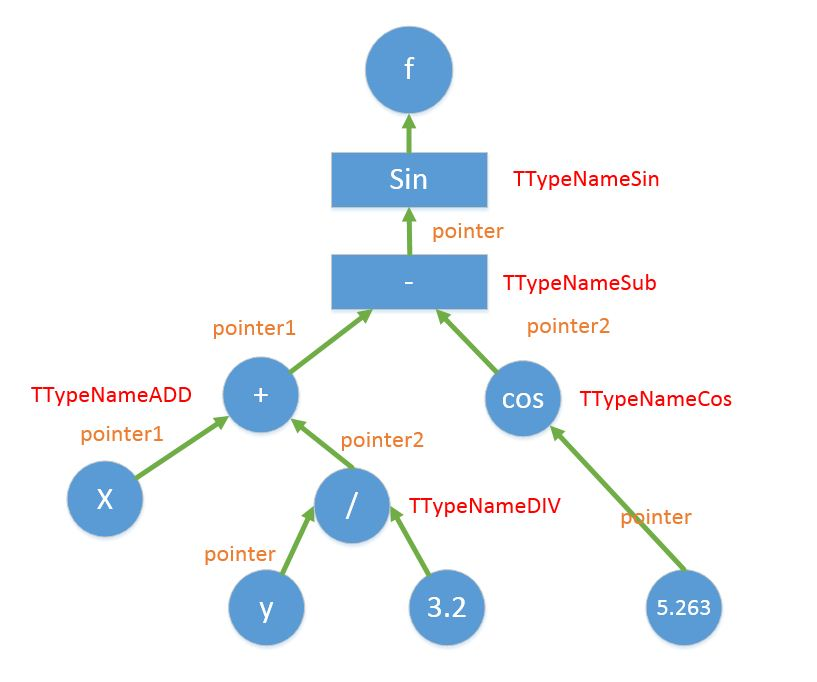
\includegraphics[scale=0.55]{images/DAG2}
	\caption{Directed Acyclic Graph in ExampleTAD1}
	%\label{FDD}
\end{figure}
Finally, we check the difference using the max norm between mpreal and double to verify the correctness of the modification. The output is
\newpage
\lstinputlisting{\OUTDIR/ExampleTAD1_result.txt}
%\section{An application using the Tadiff to solve an ODE}
%{\textbf{In ExampleTAD2.cpp}}
%\lstinputlisting{\SRCDIR/ExampleTAD2.cpp}
%In this example, we use the Taylor-expansion template to solve an ODE which is a possible applicaton for the Taylor-expansion template. The recorded DAG connecting two instance variables in the class TODE is simple below:
%\begin{figure}[H]
%	\centering
%	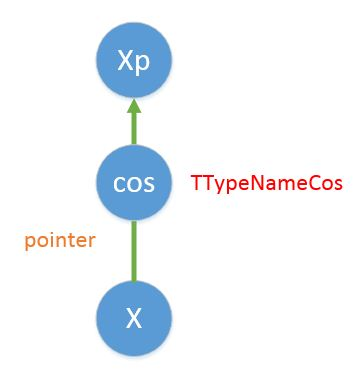
\includegraphics[scale=0.5]{images/DAG3}
%	\caption{DAG in class TODE}
%\end{figure}
%The output is shown below:
%\lstinputlisting{\OUTDIR/ExampleTAD2_result.txt}
\newpage
\section{Makefile}
The overall makefile to make all the example executives is shown below:
\lstinputlisting{\SRCDIR/makefile}